% Results section

The results from the NIST benchmark suite for each individual device are
displayed in figure \ref{fig:nist_results}.  Additionally, the measured
bitrates for each device are listed in figure \ref{fig:bitrates}.

\begin{figure}[h]
	\centering
	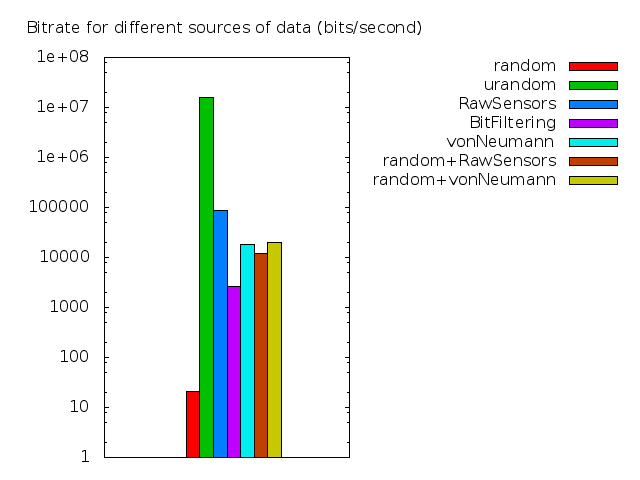
\includegraphics[width=0.5\textwidth]{bitrate.png}
	\caption{Observed bitrate in bits per second.  Note that the y-axis is 
a logarithmic scale.}
	\label{fig:bitrates}
\end{figure}

As shown in the graphs, any form of raw data not mixed into the entropy pool
with other sources of entropy and hashing is not suitable for use as a source
of random bits.  While the bitrates from the raw sensor data (accelerometer
and gyroscope data combined) are relatively high, these bits fail most of the
NIST tests.  With bit filtering, the proportion of tests that passed is higher
than for the raw data, but overall the data does not prove to be statistically
sound.  Data extracted using von-Neumann whitening is similarly characterized -
a slightly larger proportion of tests on the data passed, but overall the data
fails the test suite.  When data is run through the entropy pool, however, the
situation improves.  The raw accelerometer and gyroscope data being fed to the
pool is sufficiently dispersed (through hashing and mixing with other random
sources) so that it becomes much more uniformly distributed; there is no
reason to apply bit filtering to data because of this.  As expected, the
von-Neumann whitened data processed in the entropy pool is statistically
uniform, passing most of the tests in the testsuite.  These results demonstrate
the strong statistical properties of mixing many independent sources using hash
functions.  Finally it is interesting to note that both the random device and
urandom device pass most of the tests.  This is to be expected, as both these
devices are designed to provide statistically uniform bits.  However, as
previously mentioned, random is a true random number source while urandom is
only a pseudo-random source.  This means more analysis is required to prove
whether data is actually random, or merely statistically uniform.  However the
NIST testsuite shows that data obtained from sensors can be used as a form of
entropy.

The bitrates for different devices indicate some interesting properties.  As
expected, the random device was slower than any other device.  However, the
obtained bitrate was much slower than expected; a bitrate of ~20 bits/second
becomes a bottleneck for any application that requires true random numbers.  It
should be noted that this rate should increase when the phone is in use (more
data is being generated, hence a larger amount of entropy).  As also expected,
the pseudo-random device had a bitrate orders of magnitude larger than any other
device.  This is because the device is CPU-bound - it does not need to wait for
any events for data to be generated.  The bitrates of the remaining devices are
intuitive; utilizing raw data from the gyroscope and accelerometer as soon as it
becomes available is faster than performing any sort of post-processing.  Bit
filtering and von-Neumann whitening are slower than simply using raw data, but
are faster than the other devices because they do not incur the overhead of
stirring the data into the entropy pool.  Finally, the devices that utilize the
entropy pool are the slowest (besides the random device, which is orders of
magnitude slower).  Interestingly, the bitrate for von-Neumann whitened data run
through the entropy pool is higher than the bitrate of the raw data run through
the entropy pool - this highlights the indeterministic nature of the entropy
pool.  While this graph indicates a hierarchy of bitrates, many of these devices
provide data that is unacceptable for use in cryptographic applications.  For
example, even though the raw accelerometer and gyroscope data can be provided
at a higher bitrate than several of the other sources, the bits obtained fail
almost every single statistical test.  This stresses the importance of finding a
balance between the quantity and quality of random data obtained from these
devices, possibly based on the needs of the application.
